% !TEX program = pdflatex
% !TEX spellcheck = en_US
%
% FEMMX Qt GUI (femmqt) User's Manual.
% Companion to manual/manual.tex (the classic MFC GUI manual) -- this
% document covers only the new Qt6-based GUI (femmqt.exe), which as of
% this writing supports Magnetics and Heat Flow problems sharing one
% geometry editor, one Materials library, and the same property-list
% workflow. Built with a plain pdflatex pipeline (native PNG support,
% no dvips/Ghostscript step) -- see build_manual.bat.
\documentclass[11pt]{report}

\usepackage[letterpaper,margin=1in]{geometry}
\usepackage{graphicx}
\usepackage{float}
\usepackage{enumitem}
\usepackage{xcolor}
\usepackage{hyperref}
\usepackage{parskip}

\graphicspath{{images/}}

\hypersetup{
  colorlinks=true,
  linkcolor=blue!50!black,
  urlcolor=blue!50!black,
  citecolor=blue!50!black,
  pdftitle={FEMMX Qt GUI User's Manual},
  pdfauthor={FEMMX Project}
}

% Every figure in this manual is small and directly tied to the
% paragraph that introduces it, so pin them with [H] rather than
% letting LaTeX's float algorithm drift them onto later pages.
\newcommand{\dlgfig}[2]{%
  \begin{figure}[H]
    \centering
    \includegraphics[width=0.55\textwidth,keepaspectratio]{#1}
    \caption{#2}
  \end{figure}
}
\newcommand{\winfig}[2]{%
  \begin{figure}[H]
    \centering
    \includegraphics[width=0.9\textwidth,keepaspectratio]{#1}
    \caption{#2}
  \end{figure}
}

\title{\LARGE FEMMX Qt GUI\\[8pt]\Large A Modern Interface for Magnetics and Heat Flow\\[8pt]\large User's Manual}
\author{}
\date{\today}

\begin{document}

\begin{titlepage}
\centering
\vspace*{2in}
{\LARGE FEMMX Qt GUI (femmqt)\par}
\vspace{16pt}
{\Large A Modern Interface for Magnetics and Heat Flow Analysis\par}
\vspace{24pt}
{\large Version 2.1.0\par}
\vspace{8pt}
{\large User's Manual\par}
\vspace{16pt}
\today
\vspace{48pt}

\begin{minipage}{0.8\textwidth}
\centering
\small
This manual documents \texttt{femmqt.exe}, the Qt6-based graphical
interface that ships alongside FEMMX's original interface (the
``Classic GUI''). It is a companion to, not a replacement for, the main
FEMMX manual -- the underlying solvers, file formats, and Lua scripting
interface are unchanged and are documented there. This manual covers
only the Qt GUI's own windows, menus, and dialogs, and walks through
two complete worked examples: a magnetics problem, and adding a
heat-flow analysis to that same geometry.
\end{minipage}

\vfill
FEMMX project \\
\href{https://github.com/SpgV0/femmx}{\tt github.com/SpgV0/femmx}
\end{titlepage}

\tableofcontents

\chapter{Introduction}

FEMMX's Qt GUI (\texttt{femmqt.exe}) is a second, modern interface for
building and solving finite-element problems, built with Qt6 instead of
the original MFC toolkit. It is designed to feel closer to a modern CAD
program -- mouse-wheel zoom, click-and-drag selection, a real Undo, and
a resizable window -- while reading and writing the exact same file
formats the Classic GUI and command-line solvers already use.

\section{Magnetics and Heat Flow, one workflow}

The Qt GUI currently supports two physics types:

\begin{itemize}
  \item \textbf{Magnetics} (\texttt{.fem} problem files, \texttt{.ans}
    solutions) -- the same planar/axisymmetric magnetics analysis as
    the rest of FEMMX.
  \item \textbf{Heat Flow} (\texttt{.feh} problem files, \texttt{.anh}
    solutions) -- steady-state thermal conduction analysis.
\end{itemize}

The key idea behind the Qt GUI is that these two physics types
\emph{share one geometry editor and one Materials library}. You draw
your nodes, segments, arcs, and block labels once. Every material in
your problem carries \emph{both} its magnetic properties (permeability,
conductivity, BH curve, \ldots) \emph{and} its heat-flow properties
(thermal conductivity, heat capacity, volumetric heat generation) in a
single, unified Material Property dialog -- if a material has no data
for one side, that side is simply left at zero, rather than being
hidden or forced to some faked default. This means a typical workflow
is: finish drawing and solving your magnetics problem, then -- reusing
the exact same geometry -- open the Heat Flow boundary/point property
lists, assign a thermal boundary condition to the same segments, save
the result as a sibling \texttt{.feh} file, and solve for temperature
without redrawing anything. The second worked example in this manual
(Chapter~\ref{ch:example-heatflow}) does exactly this.

Boundary conditions and point properties are \emph{not} unified the
same way materials are, because the two physics types' boundary
concepts are genuinely different (a magnetics ``Mixed'' boundary and a
heat-flow ``Convection'' boundary need different input fields). Instead,
each physics type gets its own boundary/point property list, but both
lists use the exact same Add/Duplicate/Edit/Delete workflow, so once you
know one you know the other.

\section{Everything you do here is optional -- the Classic GUI still works}

Nothing in the Qt GUI modifies how the Classic GUI or the command-line
solvers (\texttt{fkn.exe}, \texttt{hsolv.exe}, \ldots) behave, and files
are fully interchangeable in both directions: a \texttt{.fem}/\texttt{.feh}
file saved from the Qt GUI opens correctly in the Classic GUI, and vice
versa. A ``Switch to Classic GUI'' menu item is available from the File
menu of both the main editor and the Solution Viewer if you want to move
a file over to the older interface.

\chapter{The Main Window}

\begin{figure}[H]
  \centering
  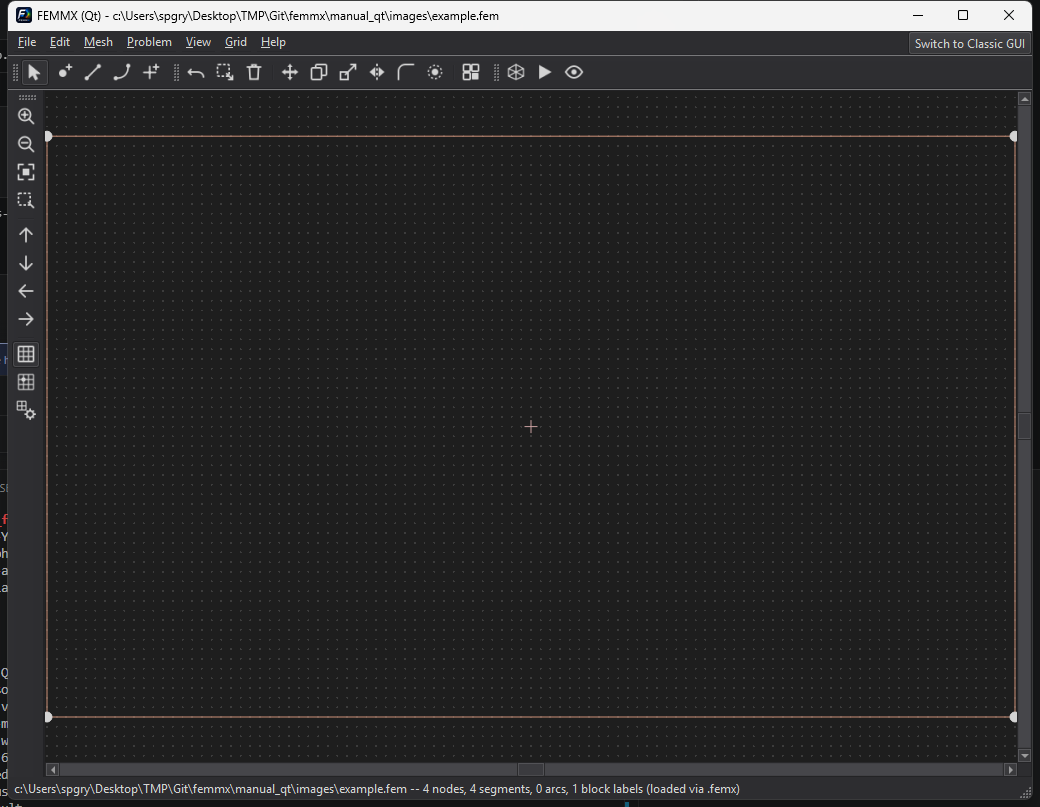
\includegraphics[width=0.9\textwidth,keepaspectratio]{00_overview.png}
  \caption{The main window: an empty problem, showing the drawing
    toolbar (left), zoom/pan/grid tool buttons (far left), and the
    six main menus.}
\end{figure}

The main window is where you build problem geometry, assign materials
and boundary conditions, and launch a solve. The left-hand toolbar
provides drawing/editing tools (Select, Add Node, Add Segment, Add Arc,
Add Block Label, Undo, Open Selected, Delete, Move, Copy, Scale,
Mirror, Create Radius, Create Open Boundary, and Select by Group),
mirroring the Edit menu described below in the same order; the
play-arrow icon solves the problem and the eye icon opens the Solution
Viewer. A narrower strip of buttons on the far left controls zoom,
pan, and the grid. Hovering over any toolbar button shows its name in
a tooltip.

\section{File menu}
\winfig{menu_file.png}{The File menu.}

\begin{description}[leftmargin=2cm,style=nextline]
  \item[New / Open\ldots / Save / Save As\ldots] Standard file
    operations for the \textbf{magnetics} (\texttt{.fem}) problem.
  \item[Open Heat Flow\ldots / Save Heat Flow / Save Heat Flow As\ldots]
    The same operations for the \textbf{heat-flow} (\texttt{.feh})
    problem sharing this window's geometry. See
    Section~\ref{sec:dual-save} for how the two save paths interact.
  \item[Import DXF\ldots / Export DXF\ldots] Import or export the
    geometry (nodes, segments, arcs) as a DXF file.
  \item[Print Preview\ldots / Print\ldots / Print Setup\ldots] Print the
    geometry view.
  \item[Recent Files] A shared list of recently opened files, for
    either physics type.
  \item[Switch to Classic GUI\ldots] Saves the current file(s) if
    needed, launches \texttt{femmx.exe} (the Classic GUI) with the same
    file open, and closes this window.
\end{description}

\subsection{Saving both a magnetics and a heat-flow file together}
\label{sec:dual-save}

The main window tracks two independent file paths: the currently open
\texttt{.fem} path and the currently open \texttt{.feh} path, since both
can refer to the same underlying geometry. Once \emph{both} paths have
been established (i.e.\ you have saved or opened both a \texttt{.fem}
and a \texttt{.feh} for this geometry), saving one opportunistically
re-saves the other too, so they never drift out of sync with each
other's copy of the shared geometry. When you use ``Save Heat Flow
As\ldots'' for the first time on a geometry that already has a saved
\texttt{.fem}, the Save dialog conveniently defaults the suggested file
name to the \texttt{.fem}'s own base name with a \texttt{.feh}
extension (Figure~\ref{fig:save-heatflow-dialog}) -- the concrete
realization of ``finish the magnetics problem, then easily add heat
flow to it.''

\begin{figure}[H]
  \centering
  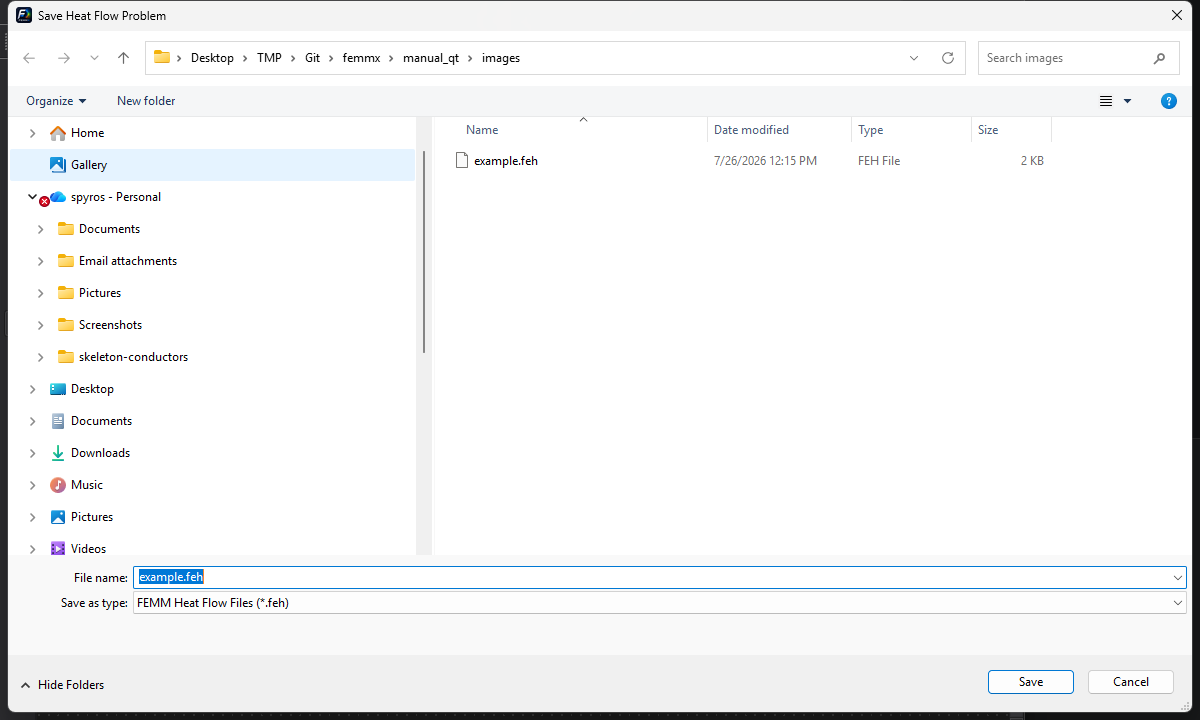
\includegraphics[width=0.75\textwidth,keepaspectratio]{save_heatflow_dialog.png}
  \caption{``Save Heat Flow As\ldots'' defaults to \texttt{example.feh}
    because \texttt{example.fem} was already saved in this folder.}
  \label{fig:save-heatflow-dialog}
\end{figure}

\section{Edit menu}
\winfig{menu_edit.png}{The Edit menu.}

\begin{description}[leftmargin=2cm,style=nextline]
  \item[Undo] Reverts the last destructive operation (a single-level
    undo, matching the Classic GUI's own behavior).
  \item[Open Selected] Opens the properties dialog for whatever is
    currently selected (equivalent to double-clicking it).
  \item[Delete] Deletes the current selection.
  \item[Move\ldots / Copy\ldots / Scale\ldots / Mirror\ldots] Geometric
    transforms applied to the current selection.
  \item[Create Radius\ldots] Fillets a corner between two selected
    segments/arcs into a smooth radius.
  \item[Create Open Boundary\ldots] Adds an asymptotic outer-boundary
    layer (the Kelvin-transform ``ABC'' technique) around the selected
    region, for problems that extend to infinity.
  \item[Copy as Bitmap] Copies the current geometry view to the
    clipboard as an image.
  \item[Select by Group\ldots / Set Group\ldots] Selects, or assigns,
    entities by their numeric group ID.
  \item[Preferences\ldots] Opens the application Preferences dialog
    (Section~\ref{sec:preferences}).
\end{description}

\section{Mesh menu}
\label{sec:mesh-menu}
\winfig{menu_mesh.png}{The Mesh menu.}

\begin{description}[leftmargin=2.5cm,style=nextline]
  \item[Create Mesh / Show Mesh / Purge Mesh] Generate, toggle the
    display of, and delete the triangular mesh, without running a
    solve.
  \item[Solve] Meshes (if needed) and solves the \textbf{magnetics}
    problem, then opens the Solution Viewer on the resulting
    \texttt{.ans}.
  \item[View Results\ldots] Opens an existing \texttt{.ans} file in the
    Solution Viewer.
  \item[Solve (Heat Flow)] The same, for the \textbf{heat-flow} problem
    sharing this geometry -- meshes and solves the \texttt{.feh},
    producing a \texttt{.anh}.
  \item[View Results (Heat Flow)\ldots] Opens an existing \texttt{.anh}
    file in the Solution Viewer.
\end{description}

Both Solve commands require the corresponding problem file
(\texttt{.fem} or \texttt{.feh}) to already be saved to disk, since the
mesher and solver are external executables (\texttt{triangle.exe}, then
\texttt{fkn.exe} or \texttt{hsolv.exe}) invoked against that file --
exactly as the Classic GUI does.

\section{Problem menu}
\label{sec:problem-menu}
\winfig{menu_problem.png}{The Problem menu. Note the single, unified
  \emph{Materials\ldots} entry near the top -- materials are shared
  between physics types, so there is no separate ``Heat Flow
  Materials'' item. Boundary Properties and Point Properties, by
  contrast, are physics-specific, so each gets its own entry.}

\begin{description}[leftmargin=3cm,style=nextline]
  \item[Problem Properties\ldots] Top-level problem settings shared by
    both physics types (Section~\ref{sec:problem-properties}).
  \item[Exterior Region\ldots] Defines an axisymmetric exterior region
    for the Kelvin-transform technique (Section~\ref{sec:exterior-region}).
  \item[Materials\ldots] The unified Materials list -- every material
    in the problem, with both magnetic and heat-flow properties
    (Section~\ref{sec:materials}).
  \item[Materials Library\ldots] Browse FEMMX's bundled material
    library and add entries to the current problem's Materials list
    (Section~\ref{sec:materials-library}).
  \item[Boundary Properties\ldots] The magnetics boundary-condition
    list (Section~\ref{sec:boundary-props}).
  \item[Circuits\ldots] The magnetics circuit list
    (Section~\ref{sec:circuits}).
  \item[Point Properties\ldots] The magnetics point-property list
    (Section~\ref{sec:point-props}).
  \item[Heat Flow Boundary Properties\ldots] The heat-flow
    boundary-condition list (Section~\ref{sec:heat-boundary-props}).
  \item[Heat Flow Point Properties\ldots] The heat-flow point-property
    list (Section~\ref{sec:heat-point-props}).
\end{description}

\section{View menu}
\winfig{menu_view.png}{The View menu.}

\begin{description}[leftmargin=2.5cm,style=nextline]
  \item[Zoom In / Zoom Out / Natural / Window] Zoom controls (the
    mouse wheel also zooms). \emph{Natural} fits the whole geometry in
    the view; \emph{Window} lets you drag a rectangle to zoom into.
  \item[Scroll Left/Right/Up/Down] Pans the view.
  \item[Show Block Names] Labels each block label with its material
    name directly on the canvas.
  \item[Show Orphans] Highlights any node not connected to a segment or
    arc, to help spot accidentally disconnected geometry.
  \item[Status Bar] Toggles the bottom status bar.
  \item[Dark Theme] Switches the whole application between light and
    dark palettes; the toolbar icons recolor to match automatically.
  \item[Load Monitor] Opens the CPU/GPU/RAM Load Monitor
    (Section~\ref{sec:load-monitor}).
\end{description}

\section{Grid menu}
\winfig{menu_grid.png}{The Grid menu.}

\begin{description}[leftmargin=2.5cm,style=nextline]
  \item[Show Grid] Toggles the dotted background grid.
  \item[Snap to Grid] When enabled, new points and dragged nodes snap
    to the nearest grid intersection.
  \item[Set Grid\ldots] Sets the grid spacing.
\end{description}

\section{Help menu}
\winfig{menu_help.png}{The Help menu.}

\begin{description}[leftmargin=2.5cm,style=nextline]
  \item[Help Topics] Opens the FEMMX manual (this document, or the main
    Classic-GUI manual, depending on what is installed).
  \item[License] Shows the license text.
  \item[About FEMMX\ldots] Shows the version number and credits.
\end{description}

\chapter{Drawing and Editing Geometry}

Geometry is built from four entity types, each with its own toolbar
button and its own Properties dialog (opened by double-clicking the
entity in Select mode, or via Edit~$\to$~Open Selected):

\section{Nodes}
Click the Add Node tool, then click anywhere on the canvas to place a
node. Double-clicking an existing node opens its Properties dialog:

\dlgfig{dlg_node_props.png}{Node Properties.}

\begin{description}[leftmargin=2.5cm,style=nextline]
  \item[X / Y] The node's coordinates; editable directly here as an
    alternative to dragging.
  \item[Point Property] Which magnetics point property (if any) is
    applied at this node (Section~\ref{sec:point-props}).
  \item[Point Property (Heat Flow)] Which heat-flow point property (if
    any) is applied at this node (Section~\ref{sec:heat-point-props}) --
    independent of the magnetics assignment above it.
  \item[In Group] The node's numeric group ID, used by Select by
    Group.
\end{description}

\section{Segments}
The Add Segment tool draws a straight line between two nodes (clicking
an empty point first places a node there). Double-clicking a segment
opens:

\dlgfig{dlg_segment_props.png}{Segment Properties.}

\begin{description}[leftmargin=2.5cm,style=nextline]
  \item[Boundary] The magnetics boundary condition applied along this
    segment (Section~\ref{sec:boundary-props}).
  \item[Boundary (Heat Flow)] The heat-flow boundary condition applied
    along this segment (Section~\ref{sec:heat-boundary-props}) --
    independent of the magnetics assignment.
  \item[Let Triangle choose mesh size / Max Segment Size] Controls how
    finely this segment is discretized by the mesher.
  \item[Hide this segment in postprocessor] Excludes the segment from
    the Solution Viewer's rendering (useful for internal construction
    lines).
  \item[In Group] The segment's numeric group ID.
\end{description}

\section{Arcs}
The Add Arc tool works like Add Segment, but after picking the two
endpoints it prompts for the arc's included angle:

\dlgfig{dlg_add_arc_prompt.png}{The Add Arc angle prompt.}

Once placed, an arc's Properties dialog offers the same fields as a
Segment's (Boundary, Boundary (Heat Flow), meshing controls, group),
plus the arc angle and maximum segment size used to discretize the
curve.

\section{Block Labels}
The Add Block Label tool drops a marker inside a closed region to
identify what material fills it (and, for magnetics, whether it
belongs to a circuit). Double-clicking a block label opens:

\dlgfig{dlg_blocklabel_props.png}{Block Label Properties.}

\begin{description}[leftmargin=2.7cm,style=nextline]
  \item[Block Type] Which material fills this region
    (Section~\ref{sec:materials}) -- this single field is used by
    \emph{both} a magnetics solve and a heat-flow solve of the same
    geometry, since materials are unified.
  \item[In Circuit] Which magnetics circuit (if any) this region
    belongs to (Section~\ref{sec:circuits}).
  \item[Let Triangle choose mesh size / Mesh Size] Controls the local
    mesh density inside this region.
  \item[Magnetization Direction (deg) / Mag.\ Direction Function
    (Lua, optional)] For permanent-magnet materials: a fixed
    magnetization angle, or an optional Lua expression for a spatially
    varying one.
  \item[Number of Turns] For regions inside a circuit, how many times
    the circuit's current effectively passes through this block
    (positive or negative, for winding direction).
  \item[In Group] The block label's numeric group ID.
  \item[Is an external region label (axisymmetric)] Marks this label as
    the exterior (Kelvin-transformed) region for an axisymmetric open
    boundary problem.
  \item[Is the default block label] Marks this as the material used to
    fill any point not enclosed by a labeled region.
\end{description}

\chapter{Materials, Boundaries, Circuits, and Point Properties}

These four property types are each edited through the same list-based
workflow: Problem menu $\to$ (property type), giving an
Add~New/Duplicate/Edit/Delete list, then a per-type field editor.
Once defined, a property is assigned to geometry from that entity's own
Properties dialog (Chapter~2).

\section{Materials}
\label{sec:materials}

Problem $\to$ Materials\ldots opens the list of every material defined
in the current problem:

\dlgfig{dlg_materials_list.png}{The Materials list.}

Choosing Add New or Edit\ldots opens the Material Property dialog --
and this is where the ``one shared library'' design is most visible:
every material carries \emph{both} its magnetics fields \emph{and} its
heat-flow fields in the same dialog, under a \textbf{Heat Flow}
section:

\begin{figure}[H]
  \centering
  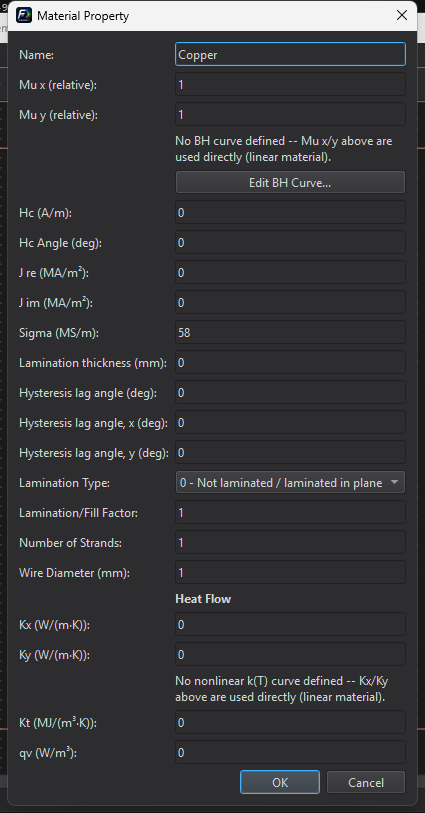
\includegraphics[width=0.42\textwidth,keepaspectratio]{dlg_material_property_unified.png}
  \caption{Material Property: a purely-magnetic material (like
    ``Copper'' fresh from the library) leaves its Heat Flow fields at
    zero.}
\end{figure}

\begin{figure}[H]
  \centering
  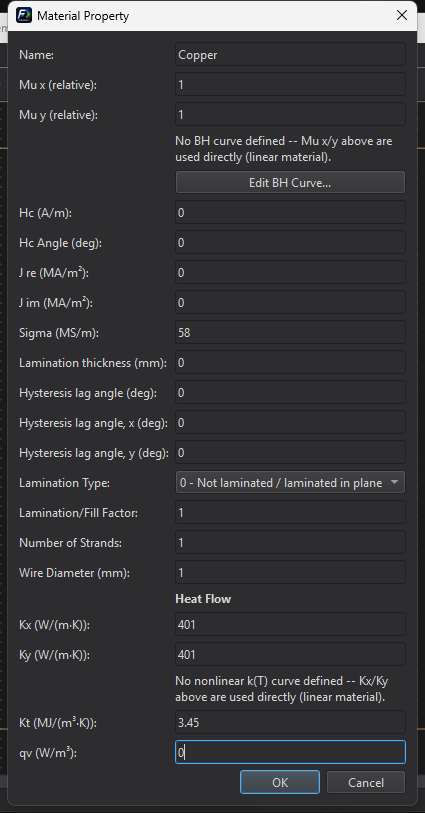
\includegraphics[width=0.42\textwidth,keepaspectratio]{dlg_material_property_filled.png}
  \caption{The same material after filling in its thermal
    conductivity ($K_x$, $K_y$) and volumetric heat capacity ($K_t$).}
\end{figure}

\begin{description}[leftmargin=2cm,style=nextline]
  \item[Mu x / Mu y (relative)] Relative permeability, or use \emph{Edit
    BH Curve\ldots} for a nonlinear material.
  \item[Hc, Hc Angle] Coercivity, for permanent magnets.
  \item[J re / J im] Applied source current density (for solid
    conductors driven directly, rather than through a circuit).
  \item[Sigma] Electrical conductivity.
  \item[Lamination thickness, Hysteresis lag angles, Lamination Type,
    Lamination/Fill Factor, Number of Strands, Wire Diameter] Fields
    controlling laminated-core and stranded-wire loss/eddy-current
    modeling -- identical in meaning to the Classic GUI's Block
    Property dialog.
  \item[Kx, Ky (W/(m$\cdot$K))] Thermal conductivity in the x and y
    directions. Leave at 0 if this material is never used in a
    heat-flow problem.
  \item[Kt (MJ/(m$^3\cdot$K))] Volumetric heat capacity (only relevant
    for transient heat-flow analyses).
  \item[qv (W/m$^3$)] Volumetric heat generation -- use this to model
    resistive/ohmic heating, chemical reaction heat, etc. See
    Chapter~\ref{ch:example-heatflow} for a worked example that sets
    this field.
\end{description}

If \emph{no} thermal data is available for a material, simply leave
its Heat Flow fields at zero -- this is a deliberate design choice
(rather than substituting some made-up default conductivity), so it is
always obvious from the dialog whether a material actually has
thermal data behind it.

\subsection{Materials Library}
\label{sec:materials-library}

Problem $\to$ Materials Library\ldots browses FEMMX's bundled
\texttt{matlib.dat}/\texttt{heatlib.dat} material database and lets you
add an entry straight into the current problem's Materials list:

\dlgfig{dlg_materials_library.png}{The Materials Library, collapsed to
  its top-level folders.}

\dlgfig{dlg_materials_library_expanded.png}{Expanding ``Solid
  Non-Magnetic Conductors'' reveals its materials.}

The library is built by merging two source files: \texttt{matlib.dat}
(magnetics properties, organized by the folders shown above) and
\texttt{heatlib.dat} (heat-flow properties for a different, and only
partially overlapping, set of material names). Where a name matches
between the two files (case-insensitively), the resulting entry carries
both sets of properties already filled in. Any \texttt{heatlib.dat}
entry that has no matching magnetics material is still made available,
grouped under a final \textbf{Heat Flow Materials (no magnetics
match)} folder, so no thermal data from the bundled library is ever
silently dropped.

\section{Boundary Properties}
\label{sec:boundary-props}

Problem $\to$ Boundary Properties\ldots manages magnetics boundary
conditions, assigned to segments/arcs from their own Properties dialog:

\dlgfig{dlg_boundary_list.png}{The Boundary Properties list.}
\dlgfig{dlg_boundary_edit.png}{Editing a Fixed-A boundary.}

The \textbf{Type} dropdown selects the boundary condition form (Fixed
A, Small Skin Depth, Mixed, Strategic Dual Image, Periodic,
Antiperiodic); the fields below it change to match whichever type is
selected.

\section{Circuits}
\label{sec:circuits}

Problem $\to$ Circuits\ldots manages named circuits, which a Block
Label can join via its \emph{In Circuit} field (with a turns count):

\dlgfig{dlg_circuits_list.png}{The Circuits list.}
\dlgfig{dlg_circuit_edit.png}{Editing a circuit.}

\begin{description}[leftmargin=2.5cm,style=nextline]
  \item[Total Amps re / im] The total current driven through the
    circuit (real and imaginary parts, for AC problems).
  \item[Circuit Type] \emph{Series} (every block sees the same total
    current, split by turns) or \emph{Parallel} (current divides
    inversely with each block's impedance).
\end{description}

\section{Point Properties}
\label{sec:point-props}

Problem $\to$ Point Properties\ldots manages magnetics point
properties, assigned to nodes from the Node Properties dialog:

\dlgfig{dlg_pointprops_list.png}{The Point Properties list.}
\dlgfig{dlg_pointprop_edit.png}{Editing a point property.}

\begin{description}[leftmargin=2cm,style=nextline]
  \item[I re / I im] A point current source at this node.
  \item[A re / A im] A fixed value of the vector potential at this
    node.
\end{description}

\chapter{Heat Flow Properties}

Heat-flow boundary conditions and point properties are edited the same
way as their magnetics counterparts (Chapter~3), just from their own
Problem-menu entries -- there is deliberately no separate ``Heat Flow
Materials''; that list is shared (Section~\ref{sec:materials}).

\section{Heat Flow Boundary Properties}
\label{sec:heat-boundary-props}

\dlgfig{dlg_heat_boundary_list_empty.png}{The Heat Flow Boundary
  Properties list, before anything has been added.}

Choosing Add New opens the editor with sensible defaults for a new,
unnamed boundary:

\dlgfig{dlg_heat_boundary_edit_default.png}{A freshly added heat-flow
  boundary, defaulting to Fixed Temperature.}

\begin{description}[leftmargin=2cm,style=nextline]
  \item[BC Type] \emph{Fixed Temperature}, \emph{Heat Flux}, or
    \emph{Convection} (mixed convective/radiative).
  \item[Tset (K)] The fixed temperature, for a Fixed Temperature
    boundary.
  \item[qs (W/m\textsuperscript{2})] The prescribed heat flux, for a
    Heat Flux boundary.
  \item[h (W/(m\textsuperscript{2}K)) / Tinf (K)] The convective heat
    transfer coefficient and ambient temperature, for a Convection
    boundary.
  \item[beta / TinfRad (K)] Radiative emissivity coefficient and
    ambient radiative temperature, also for a Convection boundary.
\end{description}

Filling these in for a convective boundary to ambient air looks like
this:

\dlgfig{dlg_heat_boundary_edit_filled.png}{An ``Ambient Air'' convective
  boundary: $h=25\,\mathrm{W/(m^2K)}$, $T_\infty=293\,\mathrm{K}$.}

\dlgfig{dlg_heat_boundary_list.png}{The list after adding it.}

\section{Heat Flow Point Properties}
\label{sec:heat-point-props}

\dlgfig{dlg_heat_point_list_empty.png}{The Heat Flow Point Properties
  list, before anything has been added.}
\dlgfig{dlg_heat_point_edit.png}{Editing a heat-flow point property.}

\begin{description}[leftmargin=2cm,style=nextline]
  \item[Tp (K)] A fixed point temperature at the node this property is
    assigned to.
  \item[qp (W)] A point heat source at that node.
\end{description}

\chapter{Problem-Level Settings}

\section{Problem Properties}
\label{sec:problem-properties}

Problem $\to$ Problem Properties\ldots edits settings that apply to
the whole geometry, regardless of which physics type you solve for
(length units, mesh refinement, precision) alongside a few
magnetics-only fields (frequency, AC solver choice) that are simply
ignored when solving for heat flow, since heat flow here is
steady-state only:

\dlgfig{dlg_problem_properties.png}{Problem Properties.}

\begin{description}[leftmargin=2.7cm,style=nextline]
  \item[Problem Type] Planar or Axisymmetric.
  \item[Length Units] The units nodes' X/Y coordinates are given in.
  \item[Frequency (Hz)] The AC excitation frequency for a magnetics
    solve (0 for a magnetostatic/DC problem).
  \item[Smart Mesh] Enables automatic mesh refinement near sharp
    corners.
  \item[Depth] The out-of-plane depth used to scale integral
    quantities (planar problems only).
  \item[Precision] The linear solver's convergence tolerance.
  \item[Min Angle] The minimum triangle angle the mesher is asked to
    maintain.
  \item[AC Solver] \emph{Successive Approximation} or a direct solve,
    for AC magnetics problems.
  \item[GPU Accel] Requests the CUDA-accelerated linear solve, if the
    installed solver executables were built with CUDA support.
  \item[Prev Type / Prev Solution] References a previous solution to
    use as the starting point (for nonlinear time-stepping problems).
  \item[Comment] A free-text description saved with the file.
\end{description}

\section{Exterior Region}
\label{sec:exterior-region}

Problem $\to$ Exterior Region\ldots defines the parameters used by the
Kelvin-transform asymptotic boundary condition (paired with a Block
Label marked ``Is an external region label'' and a boundary/segment set
up via Edit~$\to$~Create Open Boundary\ldots):

\dlgfig{dlg_exterior_region.png}{Exterior Region Properties.}

\section{Preferences}
\label{sec:preferences}

Edit $\to$ Preferences\ldots controls a few application-wide defaults:

\dlgfig{dlg_preferences.png}{Preferences.}

\begin{description}[leftmargin=2cm,style=nextline]
  \item[Use smart mesh refinement by default] The initial value of new
    problems' Smart Mesh setting.
  \item[Open XY plots in a separate window] Whether Plot X-Y
    (Section~\ref{sec:plotxy}) opens as its own window or docks inline.
  \item[Show the Output Window] The Solution Viewer's Output Window
    default visibility.
  \item[Dark theme] The application's default color theme.
\end{description}

\section{CPU/GPU/RAM Load Monitor}
\label{sec:load-monitor}

View $\to$ Load Monitor opens a live strip-chart of CPU, RAM, and (if
present) GPU utilization, with green/red markers showing when a solve
started and finished -- useful for judging how much of a long solve is
actually using the GPU accelerated path:

\winfig{view_loadmonitor_check.png}{The Load Monitor, docked over the
  geometry view.}

\chapter{The Solution Viewer}
\label{ch:solution-viewer}

Solving a problem (or choosing View Results\ldots/View Results (Heat
Flow)\ldots) opens the Solution Viewer, a dedicated window for
inspecting a solved mesh. Its menu bar and toolbar are independent of
the main editor's.

\section{File menu}
\winfig{sv_menu_file.png}{The Solution Viewer's File menu, shown over a
  density plot of $|B|$ from the magnetics worked example
  (Chapter~\ref{ch:example-magnetics}).}

\begin{description}[leftmargin=2.7cm,style=nextline]
  \item[Open Solution\ldots / Open Heat Flow Solution\ldots] Opens an
    \texttt{.ans} or \texttt{.anh} file directly.
  \item[Reload] Re-reads the current solution file from disk.
  \item[Print Preview\ldots / Print\ldots / Print Setup\ldots] Print
    the current plot.
  \item[Recent Files] Shares its list with the main editor's.
  \item[Switch to Classic GUI\ldots] Reopens the same solution in the
    Classic GUI's post-processor.
\end{description}

\section{Edit menu}
\winfig{sv_menu_edit.png}{The Edit menu.}

Copy as Bitmap copies the current plot to the clipboard as an image.

\section{Zoom menu}
\winfig{sv_menu_zoom.png}{The Zoom menu.}

Zoom In/Out/Natural and Scroll Left/Right/Up/Down work the same as
their main-editor counterparts.

\section{View menu and plot modes}
\winfig{sv_menu_view.png}{The View menu, over a Contour Plot -- the
  equipotential ($A$) contour lines of the same coil problem.}

\begin{description}[leftmargin=2.7cm,style=nextline]
  \item[Density Plot / Contour Plot] The two main plot modes. Density
    Plot fills each element with a color from a legend according to
    the selected quantity; Contour Plot instead draws lines of constant
    value, which for a magnetics solution are the field's flux lines,
    and for a heat-flow solution are isotherms.
  \item[Density Quantity] Which scalar quantity the Density Plot color
    scale represents -- $|B|$, $B_{re}$, $B_{im}$, $\log_{10}|B|$,
    $|H|$, or $|J_s+J_e|$ for a magnetics solution. (A heat-flow
    solution's Density Plot always shows the magnitude of the heat
    flux vector, labeled accordingly in the legend -- see
    Chapter~\ref{ch:example-heatflow}.)
  \item[Density Plot Options\ldots] Customize the legend's color range.
  \item[Smoothing] Blends each triangle's color from its corner nodes'
    averaged values, instead of showing one flat color per element.
  \item[Show Mesh / Show Points / Show Field Arrows] Overlay the
    triangular mesh, mesh nodes, or a fixed-length vector plot of the
    field's direction.
  \item[Show Legend] Toggles the color-scale legend.
  \item[Circuit Props\ldots] For a magnetics solution: shows computed
    current, voltage, flux linkage, and power for a circuit
    (Section~\ref{sec:sv-circuit-props}). Not applicable to a
    heat-flow solution.
  \item[BH Curves\ldots] Shows the BH curve of a nonlinear material
    used in the solution. Not applicable to a heat-flow solution.
  \item[Problem Info\ldots] Shows a summary of the solved problem's
    settings and property counts.
  \item[Output Window / Status Bar / Dark Theme] Same toggles as the
    main editor.
\end{description}

\section{Operation menu -- Point, Contour, and Area tools}
\winfig{sv_menu_operation.png}{The Operation menu.}

\begin{description}[leftmargin=2.5cm,style=nextline]
  \item[Point Properties] Click anywhere in the mesh to read off the
    interpolated field value at that exact point.
  \item[Contours] Click a sequence of points to draw a polyline across
    the mesh; use \emph{Finish Contour} (below) to report its length
    and the field difference between its two endpoints.
  \item[Areas] Click inside a block-label region to report its area and
    the area-weighted average field magnitude across every element that
    shares that label.
  \item[Finish Contour / Clear Contour] Completes or discards the
    contour currently being drawn.
\end{description}

\subsection{Circuit Properties}
\label{sec:sv-circuit-props}

\dlgfig{sv_circuit_props.png}{Circuit Properties for the ``Coil
  Circuit'' from the magnetics worked example: 5\,A total current, with
  the resulting voltage drop, flux linkage, and impedance.}

\section{Plot X-Y}
\label{sec:plotxy}
\winfig{sv_plotxy_chart2.png}{Plot X-Y along a drawn contour, showing
  $|A|$ sampled along its length.}

After drawing a contour with the Contours tool, Plot~X-Y samples a
chosen field quantity at evenly spaced points along it and displays the
result as a chart (switchable to a raw data table), exportable as a PNG
image or a CSV file.

\section{Integrate menu}

A convenience alias for the same contour-integral result shown by
Finish Contour, exposed as its own top-level command.

\section{Help menu}
\winfig{sv_menu_help.png}{The Solution Viewer's Help menu.}

\chapter{Worked Example: A Coil Cross-Section (Magnetics)}
\label{ch:example-magnetics}

This example builds a small magnetostatic problem from scratch: a
$100\,\mathrm{mm}\times 60\,\mathrm{mm}$ rectangular cross-section of a
current-carrying coil, surrounded by a fixed-boundary condition, solved
for its magnetic field. Chapter~\ref{ch:example-heatflow} continues
this same example by adding a heat-flow analysis of the coil's resistive
heating, reusing this exact geometry.

\begin{enumerate}
  \item \textbf{Draw the geometry.} Using the Add Node tool, place four
    nodes at $(0,0)$, $(100,0)$, $(100,60)$, and $(0,60)$ (all in
    millimeters). Using the Add Segment tool, connect them into a
    closed rectangle: $(0,0)\to(100,0)\to(100,60)\to(0,60)\to(0,0)$.
  \item \textbf{Define materials.} Open Problem $\to$ Materials
    Library\ldots and add ``Air'' and a solid ``Copper'' to the
    problem's Materials list (Section~\ref{sec:materials-library}).
  \item \textbf{Define a boundary condition.} Open Problem $\to$
    Boundary Properties\ldots, add a new boundary named ``Fixed
    A=0'' of Type \emph{Fixed A} with all fields left at zero
    (Section~\ref{sec:boundary-props}), then double-click each of the
    four segments and set its \emph{Boundary} field to ``Fixed A=0''.
  \item \textbf{Define a point property and circuit.} Open Problem
    $\to$ Point Properties\ldots and add ``Applied Current'' with
    $I_{re}=5$ (Section~\ref{sec:point-props}); double-click node
    $(0,0)$ and set its \emph{Point Property} to ``Applied Current''.
    Open Problem $\to$ Circuits\ldots and add ``Coil Circuit'', Series,
    Total Amps~re $=5$ (Section~\ref{sec:circuits}).
  \item \textbf{Place and assign a block label.} Using the Add Block
    Label tool, click once inside the rectangle (e.g.\ at
    $(50,30)$). Double-click it and set \emph{Block Type} to
    ``Copper'', \emph{In Circuit} to ``Coil Circuit'', and
    \emph{Number of Turns} to 1.
  \item \textbf{Save.} File $\to$ Save As\ldots, as \texttt{example.fem}.
  \item \textbf{Solve.} Mesh $\to$ Solve (Section~\ref{sec:mesh-menu}).
    The Solution Viewer opens automatically once the solve completes.
\end{enumerate}

\begin{figure}[H]
  \centering
  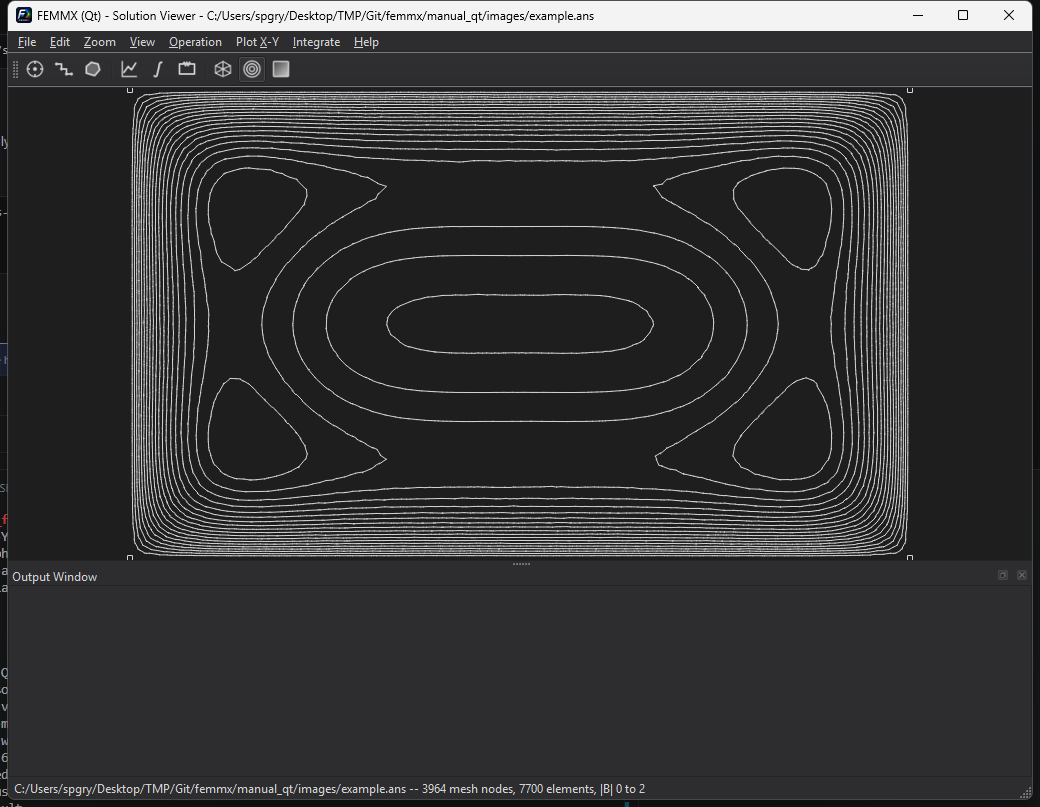
\includegraphics[width=0.75\textwidth,keepaspectratio]{sv_00_overview.png}
  \caption{The solved coil problem's default Contour Plot: field lines
    bulge symmetrically out of the coil cross-section toward the four
    fixed-$A{=}0$ walls, exactly as expected for a single conductor
    centered in a shielded rectangular boundary.}
\end{figure}

\begin{figure}[H]
  \centering
  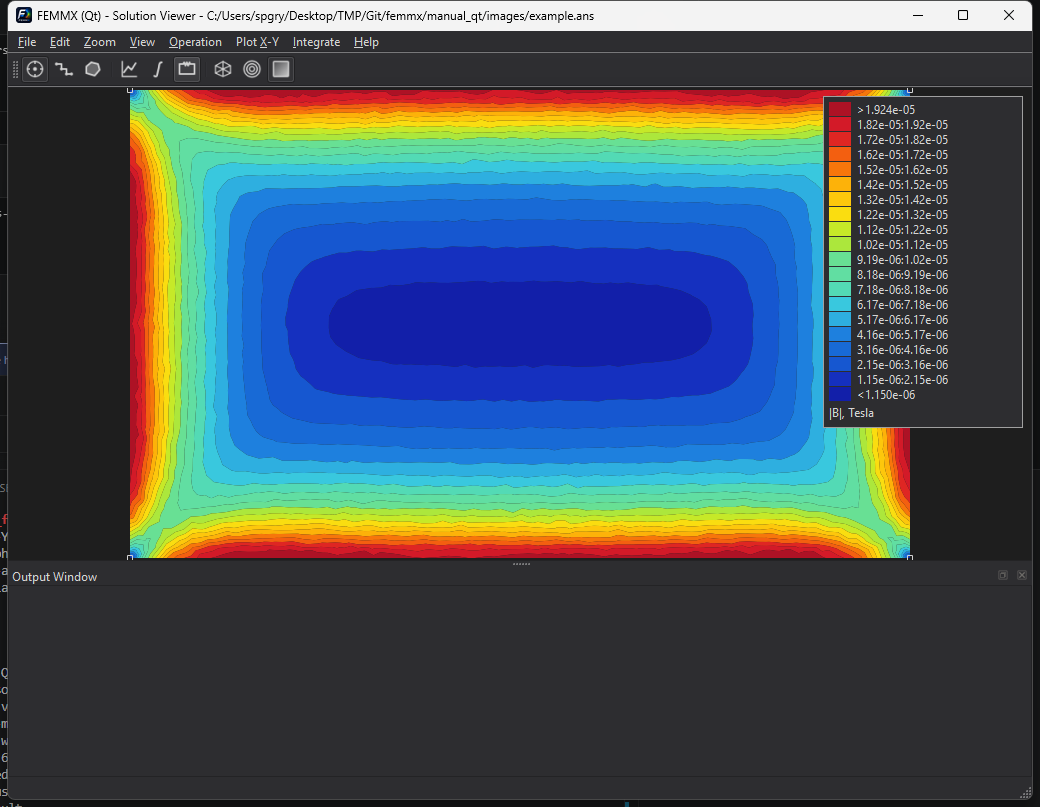
\includegraphics[width=0.75\textwidth,keepaspectratio]{sv_02_density.png}
  \caption{The same solution as a Density Plot of $|B|$: field strength
    peaks inside the conductor and falls off toward the walls.}
\end{figure}

Opening View $\to$ Circuit Props\ldots and selecting ``Coil Circuit''
confirms the circuit actually carried the 5\,A we specified, and reports
the resulting voltage drop, flux linkage, and impedance
(Figure~\ref{fig:circuit-props-recap} -- the same figure shown in
Section~\ref{sec:sv-circuit-props}).

\begin{figure}[H]
  \centering
  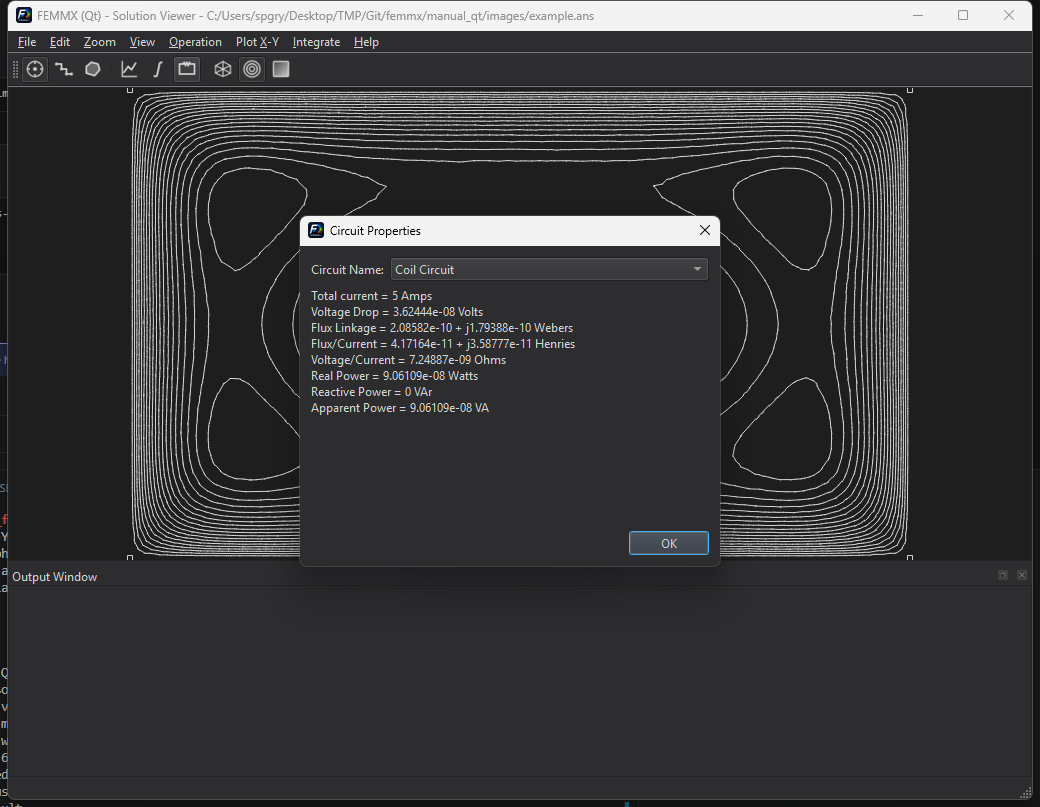
\includegraphics[width=0.6\textwidth,keepaspectratio]{sv_circuit_props.png}
  \caption{Circuit Properties for ``Coil Circuit''.}
  \label{fig:circuit-props-recap}
\end{figure}

\chapter{Worked Example: Adding Heat Flow to the Same Model}
\label{ch:example-heatflow}

Continuing directly from Chapter~\ref{ch:example-magnetics}, this
example adds a steady-state heat-flow analysis to the exact same
rectangular geometry -- modeling the coil's resistive (I$^2$R) heating,
and asking how hot its cross-section gets before that heat conducts out
to the surrounding air.

\begin{enumerate}
  \item \textbf{Start the heat-flow file.} With \texttt{example.fem}
    still open, choose File $\to$ Save Heat Flow As\ldots. Because
    \texttt{example.fem} is already saved, the dialog defaults the
    suggested name to \texttt{example.feh} in the same folder
    (Figure~\ref{fig:save-heatflow-dialog}) -- accept it. The window
    title now shows both files, and its geometry (the same rectangle,
    same block label) is shared between them.
  \item \textbf{Define a convective boundary.} Open Problem $\to$ Heat
    Flow Boundary Properties\ldots and add a new boundary named
    ``Ambient Air'', Type \emph{Convection}, with $h=25\,
    \mathrm{W/(m^2K)}$ and $T_\infty=293\,\mathrm{K}$
    (Section~\ref{sec:heat-boundary-props}).
  \item \textbf{Assign it to the boundary.} Double-click each of the
    four segments in turn and set its \emph{Boundary (Heat Flow)} field
    to ``Ambient Air'' -- leaving the segment's magnetics
    \emph{Boundary} field (``Fixed A=0'') untouched, since the two
    assignments are independent.
  \item \textbf{Add a heat source.} A coil with no dissipation and a
    boundary already at ambient temperature would solve to a trivial,
    uniform $293\,\mathrm{K}$ everywhere -- not a very illuminating
    plot. Open Problem $\to$ Materials\ldots, Edit\ldots the ``Copper''
    material, and set its \textbf{qv} field
    (Section~\ref{sec:materials}) to $2{,}000{,}000\,\mathrm{W/m^3}$, a
    representative volumetric resistive-heating rate.
  \item \textbf{Save and solve.} File $\to$ Save Heat Flow, then Mesh
    $\to$ Solve (Heat Flow). The Solution Viewer opens on the resulting
    \texttt{.anh}.
\end{enumerate}

\begin{figure}[H]
  \centering
  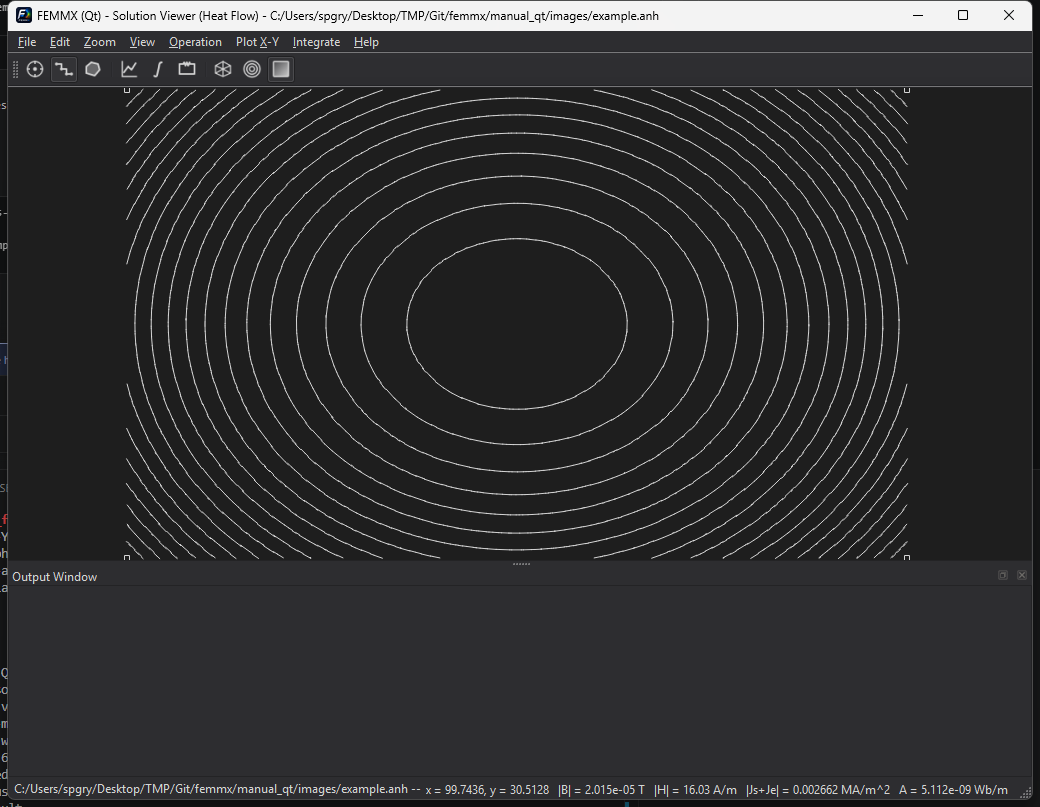
\includegraphics[width=0.75\textwidth,keepaspectratio]{sv_thermal_contour.png}
  \caption{Contour Plot of the heat-flow solution: with the Density
    Plot/Contour Plot machinery reused from the magnetics side
    (Chapter~\ref{ch:solution-viewer}), the contour lines are now
    \emph{isotherms} -- concentric rings of constant temperature,
    hottest at the copper block's center and cooling smoothly toward
    the ambient boundary on all four sides.}
\end{figure}

\begin{figure}[H]
  \centering
  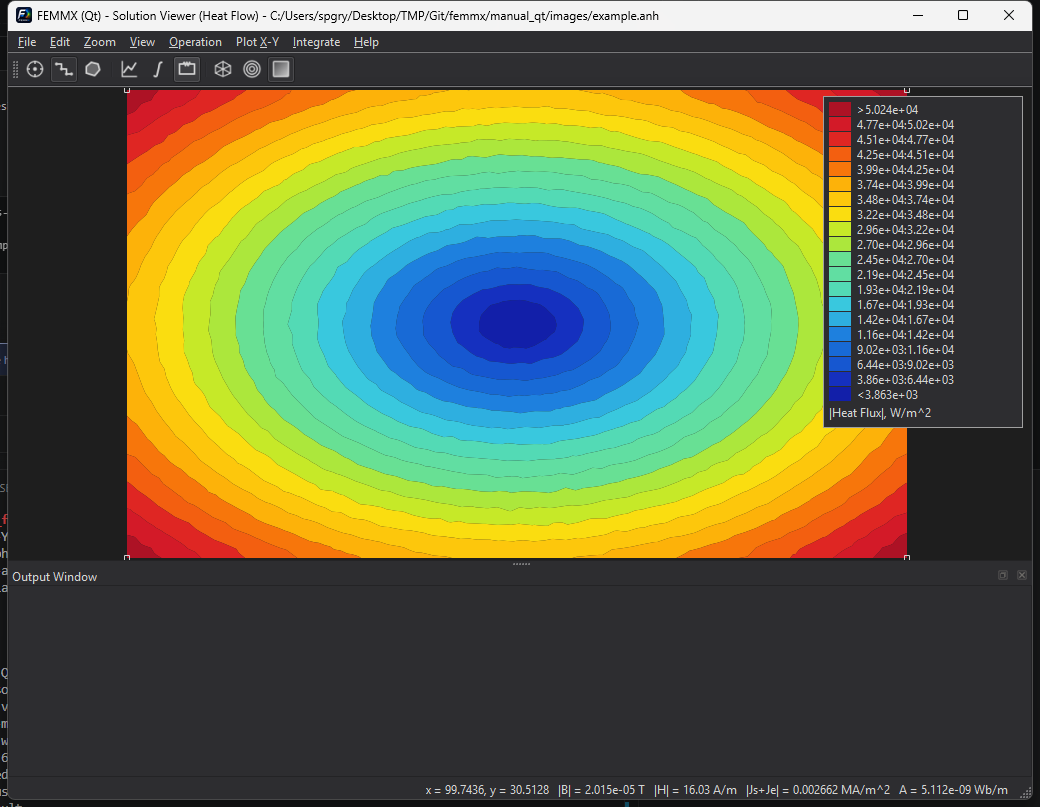
\includegraphics[width=0.75\textwidth,keepaspectratio]{sv_thermal_density.png}
  \caption{Density Plot of the same solution: this always shows
    $|\mathrm{Heat\ Flux}|$ (in $\mathrm{W/m^2}$) for a heat-flow
    result. Flux is lowest at the symmetric center (where, by symmetry,
    no net heat flows in any one direction) and highest near the
    boundary, where all of the heat generated inside must ultimately
    cross to reach the ambient air.}
\end{figure}

This is the complete pattern for combining the two physics types on one
model: draw geometry once, keep materials in one shared list, and give
each physics type its own boundary/point property assignments and its
own Solve command -- without ever having to redraw or re-import
anything between them.

\end{document}
